\subsection{Introduction} 
In this chapter it is seen how the final constellation decision is made. To do that an analysis of weighted weights will be performed.

The constellations candidates selected to their later evaluation are the following:

\subsection{Candidate 1: Polar - Global Coverage}

This polar constellation (Figure \ref{fig:Candidate1}) came from the street coverage method explained in \ref{ch:streetscov}. It is a network of polar orbits that provides global coverage. Its characteristics orbit parameters are the following:

\begin{itemize}
\item Height: $560~{km}$ 
\item Inclination of the planes: $90~{º}$  
\item Number of planes: 20
\item Number of satellites per plane: 21
\item Total number of satellites: 420
\item Range of argument of ascending node: $360~{º}$ 
\end{itemize}


\subsection{Candidate 2: Polar - GS Coverage}
 
The second candidate that will be compared is a polar orbit extracted from the coverage method explained in \ref{ch:streetscov}(Figure \ref{fig:Candidate2}). This constellation provides total coverage to the Astrea's team ground stations. The network orbits parameters are:

\begin{itemize}
\item Height: $550~{km}$ 
\item Inclination of the planes: $90~{º}$  
\item Number of planes: 18
\item Number of satellites per plane: 16
\item Total number of satellites: 288
\item Range of argument of ascending node: $360~{º}$ 
\end{itemize}


\subsection{Candidate 3 and 4: Walker-Delta GS Coverage}

Two Walker-Delta constellation configurations have been also chosen due to their reduced number of planes and satellites while being able of providing total coverage on the lattitudes where the ground stations are located.(Figures \ref{fig:Candidate3} and \ref{fig:Candidate4}).

This constellations have been obtained with the algorithm explained in \ref{Testing}

\subsubsubsection*{Candidate 3}
\begin{itemize}
\item Height: $542~{km}$ 
\item Inclination of the planes: $72~{º}$  
\item Number of planes: 8
\item Number of satellites per plane: 21
\item Total number of satellites: 168
\item Range of argument of ascending node: $210~{º}$ 
\end{itemize}

\subsubsubsection*{Candidate 4}  
\begin{itemize}
\item Height: $542~{km}$ 
\item Inclination of the planes: $72~{º}$  
\item Number of planes: 9
\item Number of satellites per plane: 17
\item Total number of satellites: 153
\item Range of argument of ascending node: $225~{º}$
\end{itemize}

\subsection{Candidate 5: Walker-Delta Lat: 0-58}

Another Walker-Delta constellation has been selected with the criteria of total coverage of a range of lattitudes going from 0 to 58 (Figure \ref{fig:Candidate5}). Therefore the parameters needed to fulfill this particular condition of the constellation obtained from \ref{ch:PerformanceAnal} are the following:

\begin{itemize}
	\item Height: $560~{km}$ 
	\item Inclination of the planes: $72~{º}$  
	\item Number of planes: 14
	\item Number of satellites per plane: 19
	\item Total number of satellites: 226
	\item Range of argument of ascending node: $210~{º}$
\end{itemize}

\subsection{Candidate 6: Polar - Walker-Delta J2 + Rotació}

With the goal of providing constant coverage at the Ground Stations we can design a constellation that takes profit of the rotation of the Earth. If we also consider Earth's oblateness that causes another $\Omega$ derivative with time, we can exacty compute the longitudinal position of a plane after an orbit has passed. Now, if we design the constellation in a way that this deviation after an orbit matches the separation between planes, a line of satellites will always be on the GS. (Figure \ref{fig:Candidate6})

\begin{itemize}
\item Height: $560~{km}$ 
\item Inclination of the planes: $72~{º}$  
\item Number of planes: 14
\item Number of satellites per plane: 19
\item Total number of satellites: 226
\item Range of argument of ascending node: $210~{º}$
\end{itemize}

\subsection{Candidate 7: Walker-Delta GS Coverage 3}

The last configuration to be studied is a Walker-Delta constellation configuration designed to provide total coverage to the ground stations (Figure \ref{fig:Candidate7}). It came up from candidate 3 constellation adding one more plane in order to increase its global coverage and minimize the gaps. As can be seen below, its parameters are the same as candidate 3 adding a single plane.

\begin{itemize}
\item Height: $542~{km}$ 
\item Inclination of the planes: $72~{º}$  
\item Number of planes: 9
\item Number of satellites per plane: 21
\item Total number of satellites: 189
\item Range of argument of ascending node: $225~{º}$
\end{itemize}

\begin{figure}[H] %[b] % h / H / b / t
	\centering
	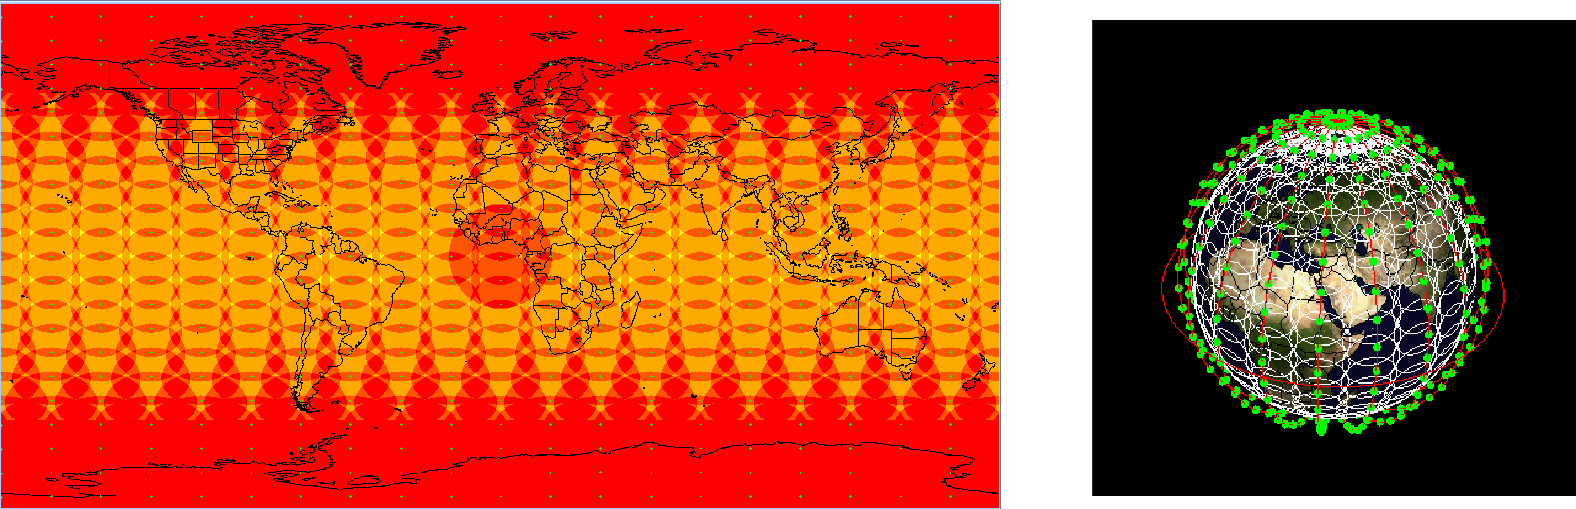
\includegraphics[width=1\textwidth]{Candidate1.png}
	\caption[Candidate 1. Full Polar constellation with global coverage]{Candidate 1. Full Polar constellation with global coverage.
			 h= 560km; Np=20; Npp=21; Tsat=420 }
	\label{fig:Candidate1}
\end{figure}

\begin{figure}[H] %[b] % h / H / b / t
	\centering
	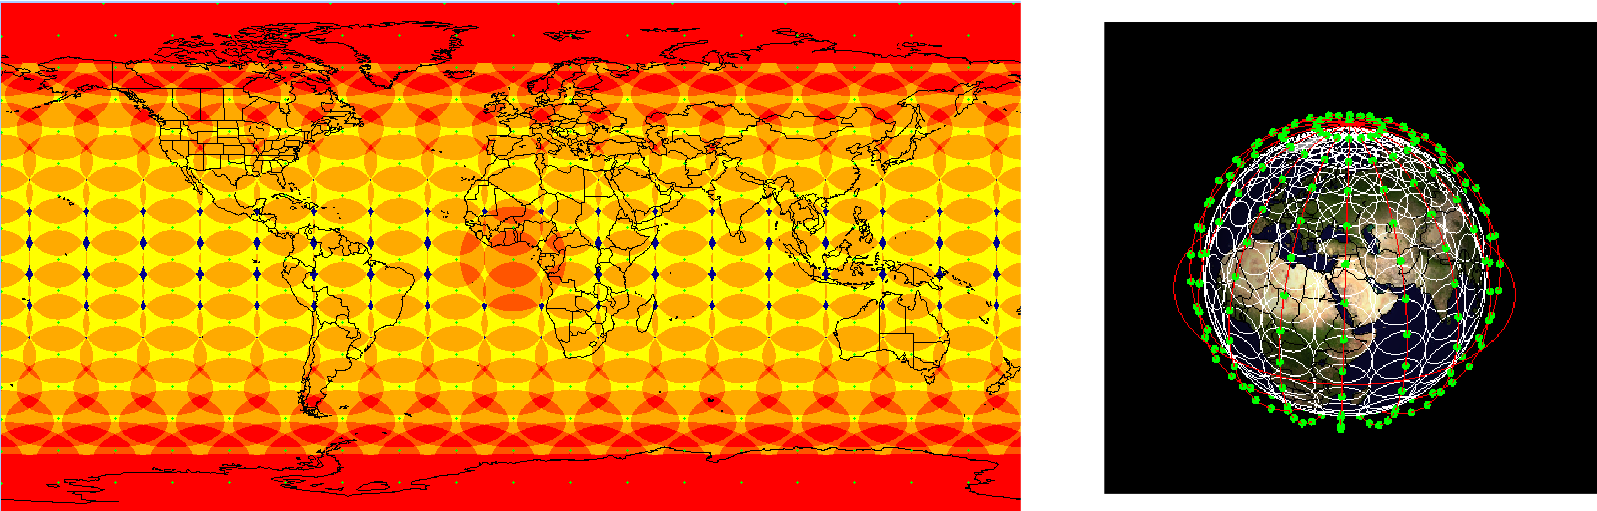
\includegraphics[width=1\textwidth]{Candidate2.png}
	\caption[Candidate 2. Full Polar constellation with total ground station coverage]{Candidate 2. Full Polar constellation with total ground station coverage.
			 h= 550km; Np=18; Npp=20; Tsat=288 }
	\label{fig:Candidate2}
\end{figure}

\begin{figure}[H] %[b] % h / H / b / t
	\centering
	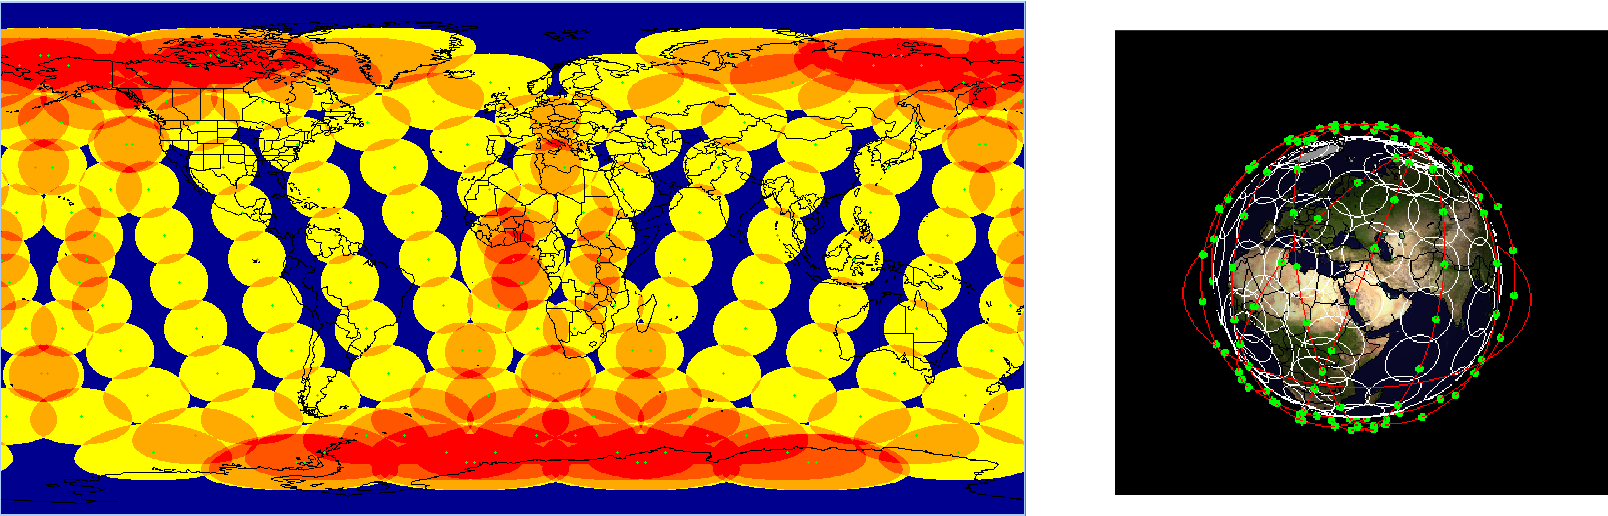
\includegraphics[width=1\textwidth]{Candidate3.png}
	\caption[Candidate 3. 210º Walker-Delta constellation configuration]{Candidate 3. 210º Walker-Delta constellation configuration.
			 h= 542km; in=72; Np=8; Npp=21; Tsat=168 }
	\label{fig:Candidate3}
\end{figure}

\begin{figure}[H] %[b] % h / H / b / t
	\centering
	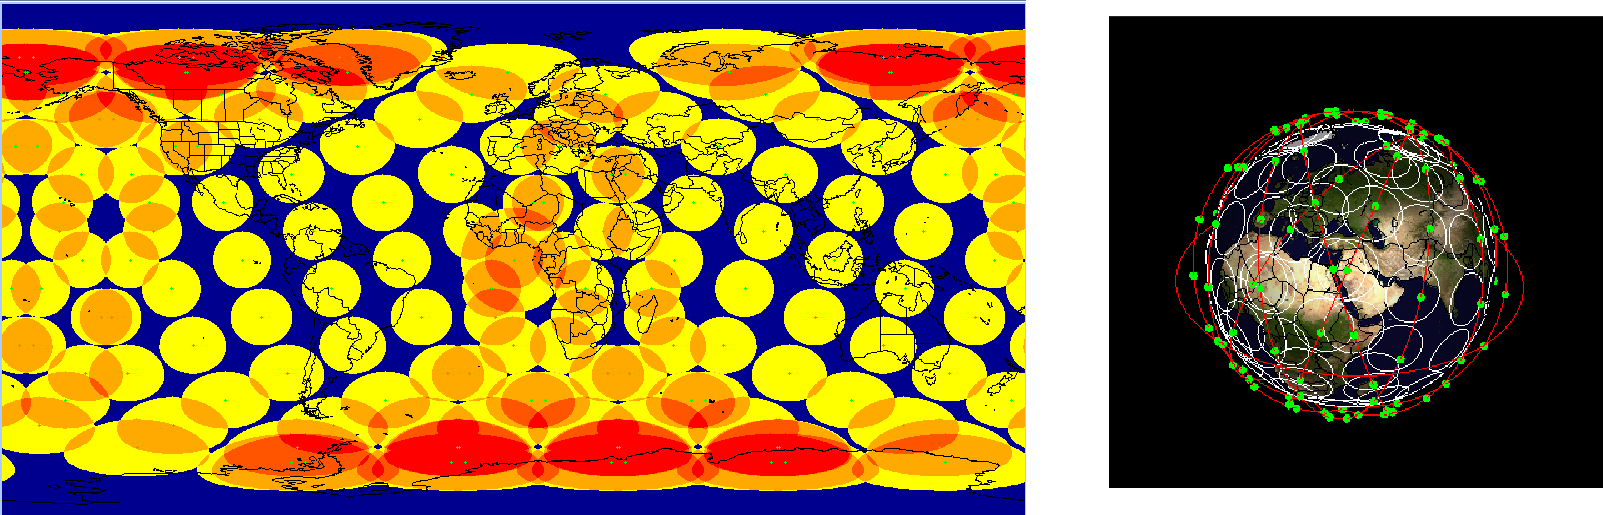
\includegraphics[width=1\textwidth]{Candidate4.png}
	\caption[Candidate 4. 225º Walker-Delta constellation configuration]{Candidate 4. 225º Walker-Delta constellation configuration.
			 h= 542km; in=72; Np=9; Npp=17; Tsat= 153}
	\label{fig:Candidate4}
\end{figure}

\begin{figure}[H] %[b] % h / H / b / t
	\centering
	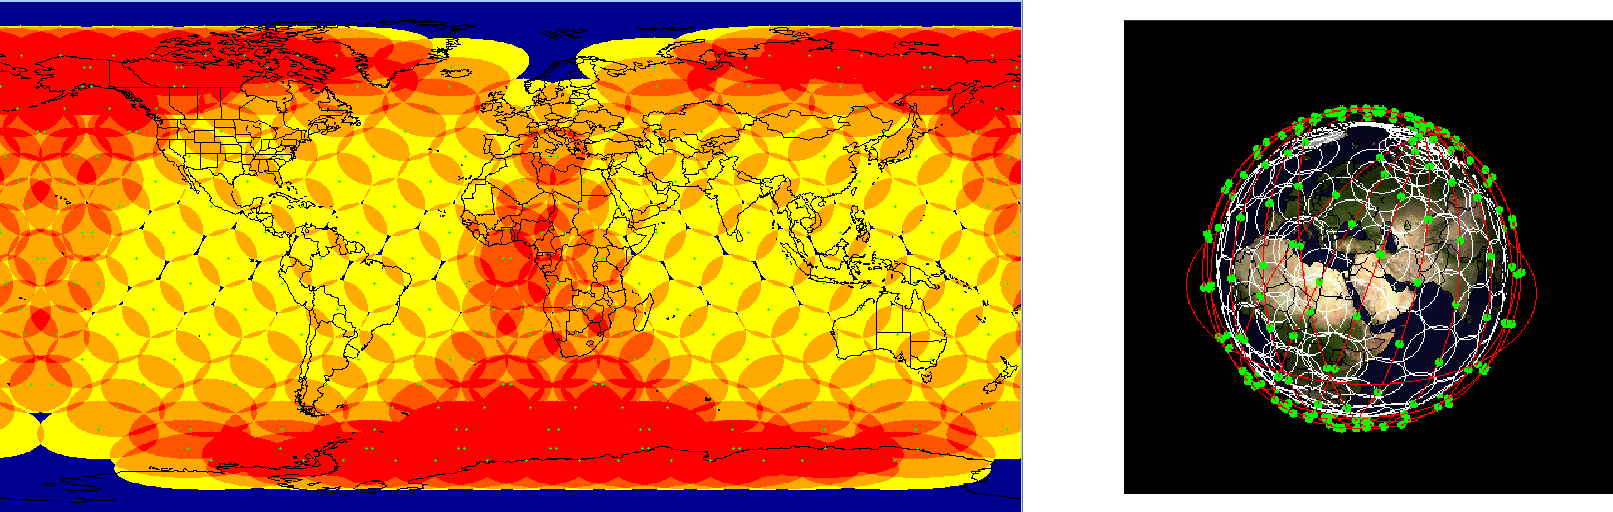
\includegraphics[width=1\textwidth]{Candidate5.png}
	\caption[Candidate 5. 210º Walker-Delta constellation configuration with total coverage of the lattitudes from 0 to 52 degrees]{Candidate 5. 210º Walker-Delta constellation configuration with total coverage of the lattitudes from 0 to 52 degrees.
			 h= 560km; in=72; Np=9; Npp=17; Tsat= 153} 
	\label{fig:Candidate5}
\end{figure}

\begin{figure}[H] %[b] % h / H / b / t
	\centering
	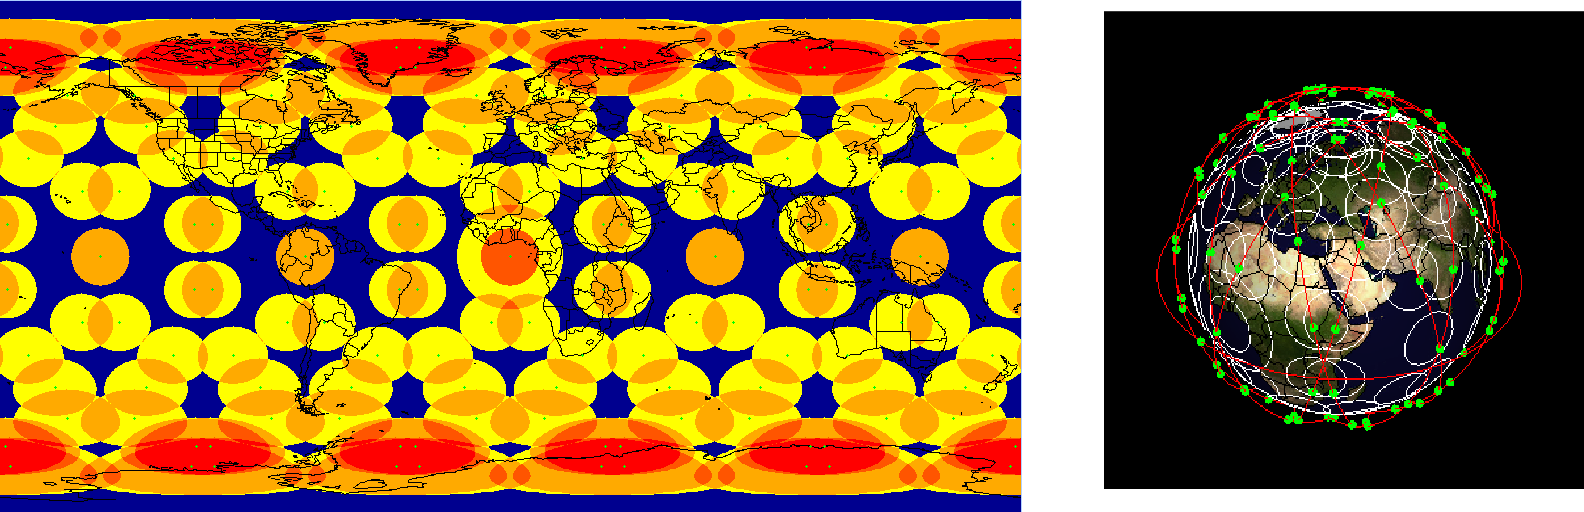
\includegraphics[width=1\textwidth]{Candidate6.png}
	\caption[Candidate 6. 225º Walker-Delta constellation configuration]{Candidate 6. 225º Walker-Delta constellation configuration.
			 h= 542km; in=72; Np=9; Npp=21; Tsat= 189}
	\label{fig:Candidate6}
\end{figure}

\begin{figure}[H] %[b] % h / H / b / t
	\centering
	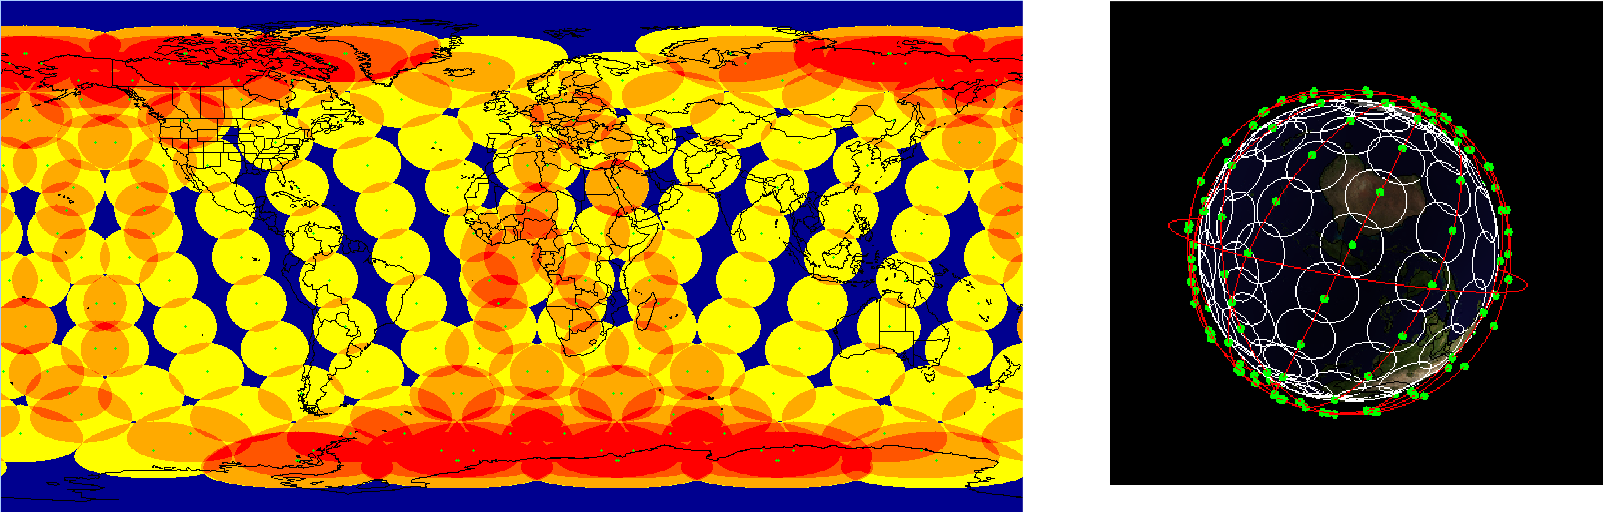
\includegraphics[width=1\textwidth]{Candidate7.png}
	\caption[Candidate 7. Full Walker-Delta constellation configuration]{Candidate 7. Full Walker-Delta constellation configuration.}
	\label{fig:Candidate7}
\end{figure}


